%%
%% 研究報告用スイッチ
%% [techrep]
%%
%% 欧文表記無しのスイッチ(etitle,eabstractは任意)
%% [noauthor]
%%

%\documentclass[submit,techrep]{ipsj}
\documentclass[submit,techrep,noauthor]{ipsj}



%\usepackage[dvips]{graphicx}
\usepackage[dvipdfmx]{graphicx}
\usepackage{latexsym}
\usepackage{url}

\def\newblock{\hskip .11em plus .33em minus .07em}

\def\Underline{\setbox0\hbox\bgroup\let\\\endUnderline}
\def\endUnderline{\vphantom{y}\egroup\smash{\underline{\box0}}\\}
\def\|{\verb|}
%

%\setcounter{巻数}{59}%vol59=2018
%\setcounter{号数}{10}
%\setcounter{page}{1}

\newcommand{\saitohcom}[1]{\textbf{{\color{blue}{[saitoh comments: #1]}}}}


%初級中級上級の手筋があることを2章に各 これについて参考文献を探す 補填は載せなくて良い こういう手筋があってその一部を紹介する


\begin{document}


\title{数独に対する最も簡単な解法探索による難易度判定付き\\ソルバー}
%(2023年7月14日版)}

%\etitle{Sudoku solver with difficulty rating by simplest solution search}%\\ (version 2023/7/14)}

%\affiliate{IPSJ}{情報処理学会\\
%IPSJ, Chiyoda, Tokyo 101--0062, Japan}

\paffiliate{KIT}{九州工業大学\\
Kyusyu Institute University}

\author{鹿屋 直大}{Naohiro Kanoya}{KIT}[kanoya.naohiro706@mail.kyutech.jp]
\author{斎藤 寿樹}{Toshiki Saitoh}{KIT}

\begin{abstract}
近年,パズルを自作し,作成したその問題を発表できるサイトの公開などにより,パズルを作成時に自分でその難易度を判断する場面が増えてきた.難易度の判定には,1つのパズルにある様々な解法の中で最も簡単なものを探す必要がある.しかし,難易度の判定を手作業で行うと,可能な限り全ての解法を考えるため,同じ問題を何度も解き直すため,多くの時間がかかってしまうとともに,見落としにより正確さも保証できない.よって,パズルの問題を入力として与えると目安となる難易度が確認できるソルバーがあるとパズル作家にとって,非常に便利である.本研究では,数独の問題を与えると,解の一意性を判定でき,最も簡単な解法を見つけ,その問題の難易度を計算するアルゴリズムを提案する.また,本提案手法により得られる難易度は本に掲載されている難易度と強い相関を持つことを示す.
\end{abstract}


%
%\begin{jkeyword}
%情報処理学会論文誌ジャーナル,\LaTeX,スタイルファイル,べからず集
%\end{jkeyword}
%
%\begin{eabstract}
%This document is a guide to prepare a draft for submitting to IPSJ
%Journal, and the final camera-ready manuscript of a paper to appear in
%IPSJ Journal, using {\LaTeX} and special style files.  Since this
%document itself is produced with the style files, it will help you to
%refer its source file which is distributed with the style files.
%\end{eabstract}
%
%\begin{ekeyword}
%IPSJ Journal, \LaTeX, style files, ``Dos and Dont's'' list
%\end{ekeyword}


\maketitle

%1
\section{はじめに}
多くのパズルは解が一意であることが重要とされる.パズルの作り手は自作の問題を作成した時に,その解の一意性を確認する必要がある.それに加え,近年では自作の問題を発表できるサイトの公開などにより,パズルの作成時に自分でその難易度を判断する場面が増えてきた\cite{PuzzleSq83:online}.しかしこれらを人間が手作業で行う場合,自分で作成した問題を自分で解き直さなければならない.特に難易度の判定には多くの時間がかかる.多くのパズルはパズルを解くためのテクニックである「手筋」をいくつか使う.それらの手筋を使う順番によって解法は異なる.パズルの難易度を判定する場合,それらの解法の中で最も簡単なものを見つけ,その解法から難易度を決定することが望まれる時がある.しかし,それを手作業で行うには同じ問題を何度も様々な解法で解いて,難易度を確認するため,多くの時間がかかり,また見落としなどが生じるため,正確に行うのも難しい.よって,問題を入力として与えると,一意性の確認と難易度の目安の出力ができるソルバーがあると便利である.

数独は株式会社ニコリの扱う代表的なペンシルパズルの1つであり,ナンバープレース(ナンプレ)など別の名前で呼ばれることもある.
数独の難易度を自動で計算する手法として,土出氏らによる手筋を見つけるのに探索したブロック,行または列の数により難易度を数値化するものがある\cite{土出智也2011数独パズルの難易度判定}.この手法は探索の中で使用する手筋の順序が決められており,適用可能な手筋を見つけるとすぐに盤面にその手筋を適用する.しかし,問題によっては,この順序に従わない別の手筋を1回適用することで盤面の多くを埋められ,適用する手筋の数を大幅に減らせることが多くあるため,多数ある解法の中で最も簡単なものを特定しているとは言えない.%これにより,解いている人がその簡単な解法で解いた場合,その人が感じる難易度と異なる可能性がある.
また,ウェブ上に公開されている難易度判定付きソルバーが存在し\cite{ペンシルパズルソ48:online},この結果を難易度の目安として出題していると見られる作り手もいる.しかしこのツールの開発者によると,これは仮置きのみを用いて解いており,その仮置きの回数をベースに難易度の点数を決めている\cite{みゃーみゃさんは39:online}.つまり,多くの人間が数独を解くときに使用する手筋を考慮せずに難易度を決めているため,実際に感じる難易度と乖離することが多くある.

本研究では,数独の問題を与えると,解の一意性を判定するとともに,その問題の難易度を計算するアルゴリズムを提案する.そのアルゴリズムは分枝限定法による手法で,問題の中から最も簡単な解法を見つけ,その解法に対する難易度を問題の難易度として計算する.%様々な解法の中から最も簡単な解法を見つけることで,見つけたところから手筋を適用するような手法にはない観点から難易度の決定を行う事ができる.
またアルゴリズムを実装し,市販の単行本に対して計算機実験を行い,問題に付けられている難易度との関係性を調べる.それにより,提案手法は土出氏らの手法よりも強い相関があることを示す.


%2
\section{数独と数独を解く手筋}

\subsection{数独}
数独のルールは以下の通りである\cite{sudoku58:online}.
	\begin{itemize}
	\item あいているマスに,1から9までの数字のどれかを入れる.
	\item タテ列 (9列ある), ヨコ列 (9列ある), 太線で囲まれた3×3のブロック (それぞれ9マスあるブロックが9つある) のどれにも1から9までの数字が1つずつ入る.
	\end{itemize}
\figref{sample_sudoku} と\textbf{~\ref{sample_sudoku_answer}} に数独の例およびその答えをそれぞれ示す.
以下では1から9までの数字が1つずつ入るマスの集合(ブロック,行,列)を\emph{領域}と呼ぶこととする.

	\begin{figure}[tb]
	\begin{minipage}[t]{0.5\columnwidth}
 	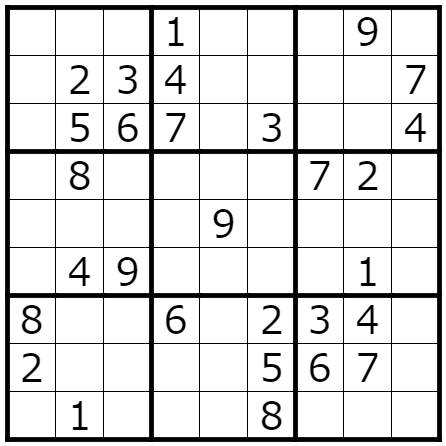
\includegraphics[keepaspectratio, scale=0.25]
      		{sample_sudoku.png}
 	\caption{数独の例}
	% \ecaption{Example of sudoku}
 	\label{sample_sudoku}
	\end{minipage}%
	\begin{minipage}[t]{0.5\columnwidth}
 	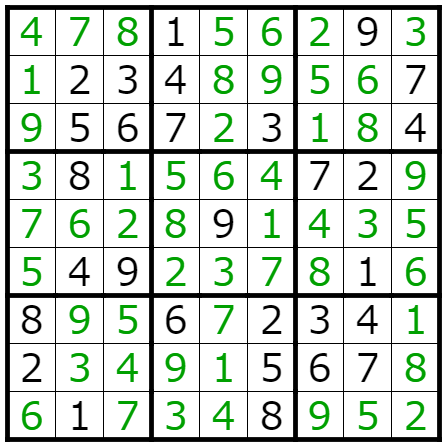
\includegraphics[keepaspectratio, scale=0.25]
      		{sample_sudoku_answer.png}
 	\caption{\figurename~\ref{sample_sudoku} の答え}
	% \ecaption{Example of sudoku - Answer}
 	\label{sample_sudoku_answer}
	\end{minipage}
  	\end{figure}
%%http://pzv.jp/p.html?sudoku_edit/9/9/i1i9h234j7g567g3h4g8j72k9k49j1g8h6g234g2j567h1i8i

\subsection{数独の手筋}

数独にはパズルを解く上で便利な手筋が知られている.手筋には初級,中級,上級のものがある~\cite{数独通信40}.
本研究が取り扱う手筋として,\emph{ブロッケン},\emph{レッツミー},\emph{マスミ},\emph{いずれにしても理論},\emph{予約},\emph{井桁理論}がある~\cite{数独通信43}.この節では,そのうち本稿で特に重要視する一部の手筋について説明する.

	\subsubsection{レッツミー}
行もしくは列内において,ある数字の入る場所が1つしかない時にその場所にその数字を入れるという手筋を\emph{レッツミー}と呼ぶ.これは中級手筋として知られている~\cite{数独通信43}.\figref{sample_rettumi}の盤面の場合,一番上の行における1の位置が\figref{sample_r_a}のように決定する.

	\begin{figure}[tb]
	\begin{minipage}[t]{0.5\columnwidth}
 	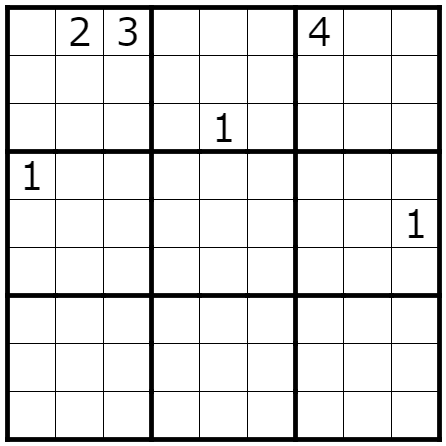
\includegraphics[keepaspectratio, scale=0.25]
      		{sample_rettumi.png}
 	\caption{レッツミーの例}
 	\label{sample_rettumi}
	%\ecaption{Example of rettumi}
	\end{minipage}%
	\begin{minipage}[t]{0.5\columnwidth}
 	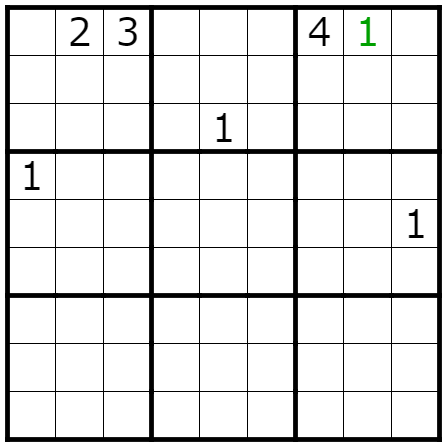
\includegraphics[keepaspectratio, scale=0.25]
      		{sample_rettumi_answer.png}
 	\caption{レッツミーの例:入れた後}
	 %\ecaption{Example of rettumi: after filling}
 	\label{sample_r_a}
	\end{minipage}
  	\end{figure}

	\subsubsection{マスミ}
あるマスにおいて,8種類の数字が同じ場所にあるため,その8種類の数字にない1つの数字をそのマスに埋める手筋を\emph{マスミ}と呼ぶ.これは中級手筋がとして知られている\cite{数独通信43}.\figref{sample_masumi}の盤面の場合,一番左上のマスが\figref{sample_masumi_answer}のように9に決定する.

	\begin{figure}[tb]
	\begin{minipage}[t]{0.5\columnwidth}
 	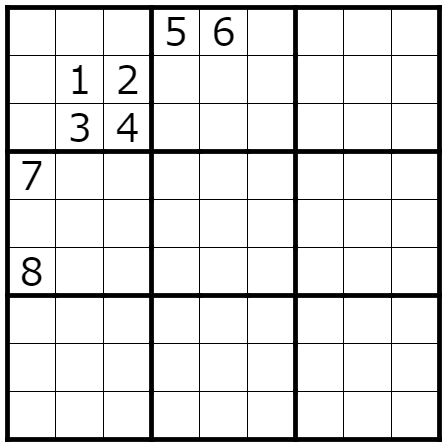
\includegraphics[keepaspectratio, scale=0.25]
      		{sample_masumi.png}
 	\caption{マスミの例}
 	\label{sample_masumi}
	 %\ecaption{Example of masumi}
	\end{minipage}%
	\begin{minipage}[t]{0.5\columnwidth}
 	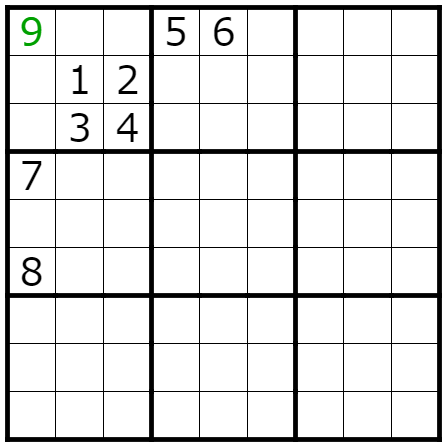
\includegraphics[keepaspectratio, scale=0.25]
      		{sample_masumi_answer.png}
 	\caption{マスミの例:埋めた後}
 	\label{sample_masumi_answer}
	 %\ecaption{Example of masumi: after filling}
	\end{minipage}
  	\end{figure}

\subsubsection{表予約}
1から9のうち2つの数字に対して,ある領域でそれらの数字が入る可能性のあるマスが,同じ2マスで重複しているときを考える.この時,その2マスにその2つの数字以外の数字は入らない.例えば\figref{yoyaku_sample}では,左上のブロックにおいて,三角で表した2つのマスは1 または 2しか入らない.これらの三角で示したマスに1,2以外の数字が入ると,三角のマス以外に 1または2を入れることになるが,それらの行もしくは列には 1 や 2 が存在してしまい,1 や 2 を入れることができない.よって,三角で示したマスに1と2以外の数字は入らない.この手筋を一般に予約と呼ぶが,ここでは次に説明する手筋と区別するために\emph{表予約}と呼ぶ\cite{数独通信43}.また,表予約は2つの数字に対するある領域の2マスだけでなく,数字とマスがそれぞれ3つから7つの場合でも成立する.

	\begin{figure}[tb]
	 \centering
 	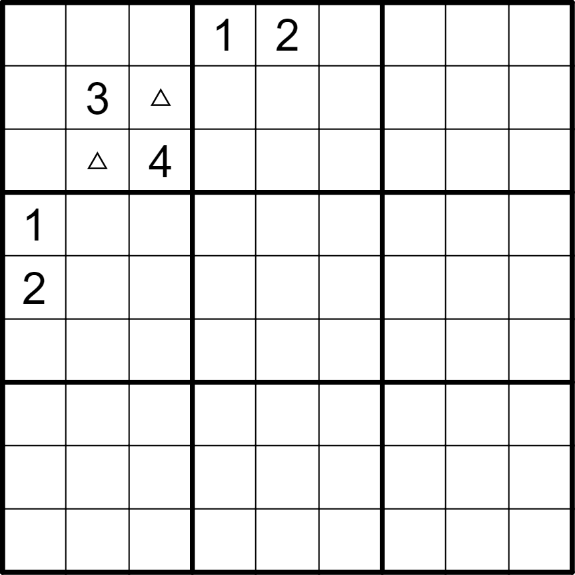
\includegraphics[keepaspectratio, scale=0.2]
      		{sample_yoyaku_blo2.png}
 	\caption{表予約の例}
	 %\ecaption{Example of front reservation}
 	\label{yoyaku_sample}
	\end{figure}

	\subsection{裏予約}
ある領域における2マスについて,そこに入る可能性のある数字がそれぞれ2つで,かつ,その2つの数字が同じである場合,その領域のその2マス以外のマスにはそれら2つの数字が入ることはない.例えば図\ref{yoyaku_sample_reverse}では,一番上の行において1マスに8と9が入っているマスが2マスある.この2マスにはどちらも8か9のいずれしか入らない.ここで,三角で示したマスに8が入ると,この2マスのいずれも9しか入らなくなり,入る数字は9に決定する.しかし,この2マスは同じ行にあるので2つの数字が同じ行に入る事になり,ルールと矛盾が生じる.三角で示したマスに9が入る場合も同様である.したがって,三角で示したマスには8と9は入らない.この手筋は「予約」と呼ばれるが,表予約と区別するために\emph{裏予約}と呼ぶ\cite{数独通信43}.また,裏予約はある領域での2マスに対する2つの数字だけでなく,マスと数字がそれぞれ3つから7つの場合でも成立する.

%https://tinyurl.com/5n7cfk9r

	\begin{figure}[hbtp]
	\setlength\textfloatsep{0pt}
 	\centering
 	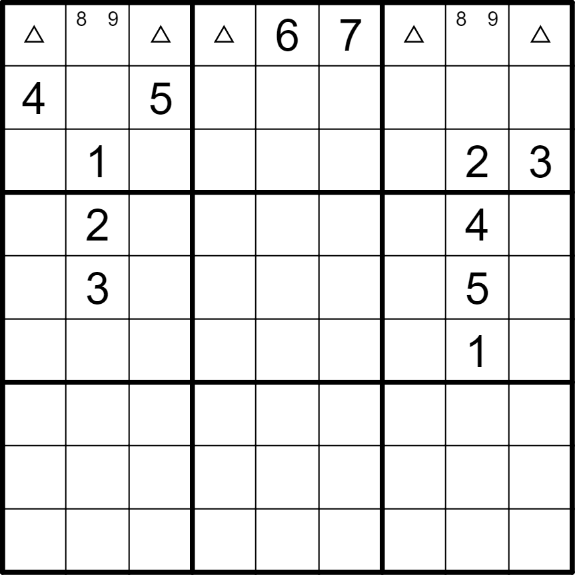
\includegraphics[keepaspectratio, scale=0.2]
      		{sample_yoyaku_reverse.png}
 	\caption{裏予約の例}
 	\label{yoyaku_sample_reverse}
	\end{figure}

%3
\section{提案手法}
本節では、数独の問題が与えられると、最も簡単な解法を探し、その解法の難易度を決定する手法を提案する.
提案手法ではまず,与えられた問題に対し,様々な手筋を用いて,問題の解の一意性をチェックするとともに,問題が初級,中級,上級のいずれであるかの分類を行う(\ref{sec:classify}節).
分類された問題に対し,分枝限定法を用いて,その問題のクラスの手筋に対する点数に応じて,最も簡単な解法を見つけ出す(\ref{sec:algo}節).
また,単純な分枝限定法では各盤面において使用可能な手筋が多い場合には計算時間がかかりすぎるため,ハッシュを用いた高速化について述べる(\ref{sec:hash}節)


\subsection{解の一意性判定と問題の分類}
\label{sec:classify}
数独の難しさを表す点数を測る前に,その問題が初級,中級,上級問題のいずれに分類する.なぜなら,それぞれの問題のクラスで扱う手筋の幅が異なっており,数独の難しさを表す点数を測る時に異なる過程を踏まなければならないからである.なお,初級問題は初級手筋のみを使う問題,中級問題は初級手筋と中級手筋のみを使う問題,上級問題は初級,中級,上級手筋を使う問題と定義する.

ここでは土出らの手法をベースとする手法で,数独の難しさを表す点数を測る前で一意解であることを確かめるとともに,問題の分類を行う.まず初期盤面で初級手筋が使える場所を探してあれば適用し,これを繰り返して全て埋まれば初級問題である.全て埋まらなければ中級手筋が使える場所を探してあれば適用を繰り返し,全て埋まれば中級問題である.全て埋まらなければ上級手筋が使える場所を探してあれば適用を繰り返し,全て埋まれば上級問題である.もしそれでも全て埋まらなければ,仮置きを使って解が一意であるかを確認する.仮置きを使って解かなければならない場合には,問題は上級問題よりも難しい問題であると出力する.また,問題の解が一意ならば一意解であることを,解が複数あれば複数解を持つことを出力する.また手筋を用いて数字を入れるときにマスへの数字の埋め方に矛盾が生じるときは,その問題には解がないので,解なしと出力する.このようにして一意解の判定と初級か中級か上級かという難易度の大まかな区別を決定している.


\subsection{問題の難易度の計算手法}
\label{sec:algo}

まず,問題の難易度の定義を行う.ここでは一意解しかもたず,初級,中級,上級のいずれかの問題に分類されているもののみを扱う.そのため,いずれかの手筋を使うことで必ず解にたどり着くことができる.解にたどり着くまでに使用した手筋の列を\emph{解法}とする.各手筋には分類された問題に応じて,正の点数を付ける.探索により解法で用いた各手筋の点数を合計した値をその\emph{解法の点数}とする.解法の点数が高ければ高いほど,その解法は難しいと考える.また,ある盤面に対し,その盤面から考えられるすべての解法の中から最も点数の小さい解法の点数を,その\emph{盤面の難易度}と定義する.数独の問題の難易度はその初期盤面の難易度とする.

本研究では分枝限定法による問題の難易度の計算を効率的に行う.
%ここに旧 3.4 節を書く
数独における盤面が与えられたとする.
この盤面に対し,その盤面で使用できる全ての手筋を探す.%必要がある.なぜなら,各盤面でどの手筋を選んだら最小の難易度点数を持つ解法となるのか探す必要があるからである.このために,各盤面ではそこで使える全ての手筋を探す.
手筋を発見したら後ほどその手筋を盤面内で適用するために,その手筋の種類,それを適用する領域,関係する数字を記録する.なお,手筋を適用しても盤面内のどのマスでも候補数字が変化しない場合がある.その場合は盤面内に変化がないならその手筋を使う事に意味が無いため,その発見した手筋は使わないこととする.%なのでこの場合手筋の実行に必要な情報の記録はされない.\saitohcom{最後の一文の意味がわからないです.(なくてもよい?)}
% 各盤面は解答された状態である最終盤面以外は数独の解答途中の盤面で,手筋を使用する前の盤面である.
分枝限定法では,盤面で使える手筋を列挙し,それを適用した盤面をそれぞれの手筋ごとで作成し,作成された盤面に対して再帰的に深さ優先で探索を行う.%適用された盤面が適用する前の盤面を親とした新しい盤面となる.
これを途中で枝刈りをされるか,すべての数字が埋められるまで続ける.また,各盤面にはその盤面から再帰的に探索した中で%その盤面から数字をすべて埋める状態までで
解法の点数が最も低いものを記録する.%この記録された点数は探索中に現在の値より難易度点数が小さくなるような解法を発見したらその点数に更新されるようになっている.

各盤面 $B$ には初期盤面からその盤面に到達するまでに使用した手筋の点数の総和 $x$ を記録する.また,盤面 $B$ に到達するまでの探索の途中で得られた解法における暫定的な最小の難易度 $x^*$ を保持しておく.ここで $x$ が $x^*$ を超える場合,その盤面 $B$ からの探索で得られるどの解法も難易度点数が $x^*$ 未満となることはない.つまり,盤面 $B$ を探索することで,よりよい解法を見つけることはできないため,盤面 $B$ を枝刈りする.
% また,手筋の使用する前の盤面から手筋を使用した後の盤面を生成する時に,使用する前の盤面が持っている現時点で最も簡単な解法の難易度点数から,使用した手筋の難易度点数を引いた数をその盤面の最も簡単な解法の初期値として持っておく.これにより,生成された盤面の初期値が0以下になった場合,最も簡単な解法が他にあるという事になる.そこからどのような解法を選んでも最も簡単な解法ではなくなるので,そこから先は探索しないことで枝刈りができる.このようにして探索を行い,最終的に一番上の盤面,つまり初期盤面の盤面に記録された難易度点数が,最も簡単な解法の難易度点数になる.

具体例を\figref{sudoku_search}に示す.ここでは盤面Aから点数3である手筋を用いて盤面Bに行き,さらに点数4である手筋を用いて数字が全て埋まった解(完成盤面C)に到達したとする.盤面Aから完成盤面Cまで行く解法の点数は 7 となる.また,盤面Aにおける暫定の難易度 $x^*$ は7以下となる.ここから,盤面Aで使える,盤面Bへの探索で用いる手筋とは異なる点数4の手筋を使って盤面Dに到達するとする.ここで,盤面Dに到達するまでにかかる点数は $x = 4$ である.%の暫定の最小点数は\{7-4=3\}となる.なぜなら,3よりも大きい点数を持つ手筋を盤面Dで使うとする.盤面Aから見た,その手筋を用いた解法の点数は4に3よりも大きい数を足す事が確定しているので7よりも大きい数となる.しかし,盤面Aから見た解法で現在最も点数が小さい解法のその点数は7である.したがって,その解法は盤面Aから見て最小の難易度点数を取らない.よって,盤面Dでの暫定の最小点数は3とすることで,3以上の手筋を盤面Dで適用させないようにしている.
次に\figref{sudoku_search}では,盤面Dから点数4の手筋を用いて盤面Eへの探索を行おうとするが,盤面 E を生成するための点数の合計は 8 で暫定の最小点数よりも大きいので枝刈りされる.

	\begin{figure}[tb]
 	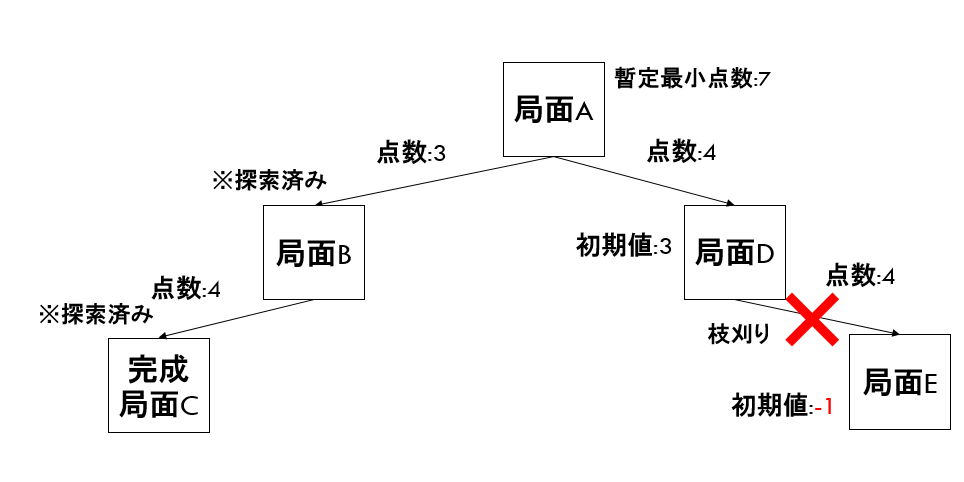
\includegraphics[keepaspectratio, scale=0.32]
      		{sudoku_search.png}
 	\caption{探索の例}
	 %\ecaption{Example of search}
 	\label{sudoku_search}
	\end{figure}

	% \subsection{手筋の列挙}

	\subsection{高速化}
\label{sec:hash}
上記の単純な分枝限定法では,各盤面で用いることのできる手筋が多い場合に探索に時間がかかる.特に上級と判定される問題がそのような盤面を多く持つ傾向にある.そのため,効率的に問題を解くためにハッシュを用いて,過去の盤面の計算結果を蓄えることでアルゴリズムの高速化を行う.
% 上級と判定された問題について,ある盤面で用いる事のできる手筋が比較的多い場合にそうでない場合と比べて探索に時間がかかったため,高速化を行った.
これは探索中に出現するある盤面 $B$ において,盤面 $B$ の難易度は,初期状態から盤面 $B$ に至るまでに使われた手筋の順番に依存しないからである.% の種類がどうであれ,一意に決定している.これが成り立つ事を説明する.
% 候補数字を含めた盤面の状態は全く同じであるが,片方は初期状態から手筋Aを用いて導かれ,もう一方は手筋Aを用いずに導かれた2つの盤面があるとする.ここで,全く同じ手筋を2回以上用いても,1回目の使用でその手筋が消す候補数字が全て消えているため盤面は変化しない.これより,手筋Aを用いて導かれた盤面について,もう一度手筋Aを使用しても盤面は変化しない.手筋Aを用いずに導かれた盤面は手筋Aを用いて導かれた盤面と候補数字まで同じであるから,手筋Aを使用しても盤面は変化しない.これより,手筋Aを用いた用いていないに関わらず,同じ盤面に対してそこから使用できる手筋の種類は同じである事が分かる.よって,初期状態からその盤面に至るまでに使われた手筋の種類がどうであれ,その盤面に対して使用できる手筋の種類は同じであるため,その盤面を解く最小点数も一意に決定している.
そのため,探索中に難易度が計算された盤面 $B$ に対して,難易度をもう一度計算することは無駄である.そこで,盤面 $B$ の難易度 $x^*_B$が計算されたら,$B$ をキーとして盤面 $B$ の難易度 $x^*_B$ をハッシュに保存する.一方で,盤面 $B$ が探索中に枝刈りされて探索が打ち切られた場合,$B$ に対する難易度は計算されていない.そのときには,その盤面をキーとして,枝刈りされた時点での初期盤面に対する暫定的な難易度 $x^*$ から今回の探索における初期盤面から $B$ を得るまでの手筋の点数の和 $x$ を引いた $x^* - x$ をハッシュに格納する.%これにより,探索中でのある盤面に対し,その盤面をハッシュで検索する事ですでに探索済みかどうかを確認することができる.%これにより,探索中でのある盤面に対し,その盤面をハッシュで検索する事ですでに探索済みかどうかを確認することができる.

ハッシュに格納された値は次のように使用する.
探索において,盤面 $B$ が作成されたとする.このとき,$B$ をキーとしてハッシュに要素が格納されているかを確認する.格納されていなければ,$B$ を根として盤面を再帰的に探索する.
$B$ が格納されているとき,ハッシュに格納されている点数 $y$ と,現在の探索における初期盤面の暫定的な難易度 $x^*$ から $B$ に到達するまでの手数の点数の和 $x$ を引いた $x^*-x$ を比べる.ここで $x^*-x \leq y$ のとき,この探索は枝刈りができる.もし,$y$ が $B$ の難易度 $x_B^*$ を表しているとすると,$B$ には $x^*-x$ よりも小さい値の解法を持たないため,その探索によって解を改善することはできない.一方で,探索済みでないとき,そのときの $y$ を上界として枝刈りを行っているため,$x^*-x$ でも同様に枝刈りが発生する.そのため,$x^*-x \leq y$ のとき,枝刈りを行う.$x^*-x > y$ のときには,再度,探索を行う.(ただし,$y=x^*_B$ とのときにはすでに計算済みであるため,計算を省くことができる.)
% 盤面と一緒に格納されている点数はそれを解くために必要な最低限の点数であることを表す.よってこの場合,現在探索中の盤面の暫定の最小の難易度点数の方が大きいため,現在探索中の盤面の最も簡単な解法の点数よりも,格納されている盤面の最も簡単な解法の難易度点数の方が小さい.したがって,難易度点数が最小となる解法を持たない盤面を探索しても無意味であるから,現在探索中の盤面に対して打ち切りを行う.そうでない場合,つまり盤面と一緒に格納されている点数が現在探索している盤面の暫定の最小難易度点数よりも大きい場合は,現在探索中の盤面の解法が最小点数を更新する可能性があるので,打ち切りをせずそのまま探索を行う.
このようにハッシュを用いて探索中に出現した盤面とそのときの値を保存し,再度現れた際の探索での枝刈りに利用することで探索を効率的に行う.
%その点数をハッシュから取り出すことで高速に求めることができる.
% 具体的には,探索中の盤面の最小点数が決定した時,もしくは探索が打ち切られた時にその盤面と点数を格納する.探索中の盤面の最小点数が決定した時は,その盤面とそれを解くための解法の最小点数の組み合わせをハッシュに格納する.この2つの場合のいずれにせよハッシュに格納された盤面に対してそれを解くための解法の最小点数は,一緒に格納された点数以上となる.
% この打ち切りにより,同じ盤面に対して何度も同じ計算をしなくてよいので,高速化を行う事ができる.



%4
\section{計算機実験}
本研究では3節で提案したアルゴリズムをプログラミング言語 C++ で実装し,計算機実験を行った.本節ではその結果を示す.本実験ではプロセッサ Intel(R) Core(TM) i7-8550U CPU @ 1.80GHz 2.00 GHzを持つ計算機を使用した.
今回は2節で名称を出した手筋が初級,中級,上級手筋のうちどれに当たるかを表~\ref{solution_point}の通りに定義する.さらに同じ公式難易度の問題がほぼ同じ点数になるように,また見つけるための難しさを考慮して,著者が感覚的に設定した.各手筋が初級,中級,上級のどれに当たるかと,各手筋の点数を表\ref{solution_point}に示している.

	\begin{table}[tb]
		\caption{各手筋の分類と点数}
		\label{solution_point}
			\begin{tabular}{ccr}
			\hline\hline
			手筋 & 難易度 & 点数[点]\\
			\hline
ブロッケン & 初級 & 0\\ 
レッツミー & 中級 & 1\\
マスミ & 中級 & 7\\
いずれにしても理論 & 上級 & 7\\
ブロック2マス表予約 & 上級 & 10\\
列2マス表予約 & 上級 & 30\\
ブロック3マス表予約 & 上級 & 40\\
列3マス表予約 & 上級 & 80\\
ブロック2マス裏予約 & 上級 & 80\\
列2マス裏予約 & 上級 & 80\\
2列の井桁理論 & 上級 & 80\\
ブロック4マス表予約 & 上級 & 90\\
列4マス表予約 & 上級 & 100\\
ブロック3マス裏予約 & 上級 & 100\\
列3マス裏予約 & 上級 & 100\\
ブロック4マス裏予約 & 上級 & 120\\
列4マス裏予約 & 上級 & 120\\
			\hline
	 	\end{tabular}
	\end{table}

\subsection{実験結果}
計算機実験におけるパズルの問題として,株式会社ニコリ社から発行されている「てごろな数独1」の,難易度Mediumの問題から問題番号が4の倍数である18問を抜粋して扱う\cite{てごろな数独1}.それらの問題に対して本研究で作成したプログラム (\emph{ours}) と,土手らの手法 (\emph{known}) による難易度判定プログラムをそれぞれ実行した.その結果,どちらの手法においてもすべての問題を効率的に解くことができ,またいずれの問題も解が一意であることが確認できた.また,それぞれの手法における,各問題に対して出力された難易度を\tabref{study_medium}に示す.
また,公式難易度は「てごろな数独1」など株式会社ニコリの一部の数独の単行本で各問に対して設定されている,1,2,3,4,5,6,7,8,8+,9,9+,10,10+の13段階で設定されている難易度を示す値である.本研究で使用する数独の単行本の問題は全てこの13段階の難易度が設定されている.
公式難易度と計算機実験により得られた難易度で相関を取ると,提案手法(ours) では相関係数は0.68となり,既存手法 (known) では相関係数は0.27 となった.
	\begin{table}[tb]
		\caption{中級問題に対する難易度}
		\label{study_medium}
			\begin{tabular}{crcr}
			\hline\hline
			問題 & ours[点] & known[点] & 公式難易度\\
			\hline
問題16 & 1 & 41 & 4\\
問題20 & 1 & 45 & 4\\
問題24 & 1 & 74 & 4\\
問題28 & 1 & 72 & 4\\
問題32 & 1 & 65 & 4\\
問題36 & 1 & 68 & 4\\
問題40 & 3 & 66 & 5\\
問題44 & 2 & 65 & 5\\
問題48 & 3 & 75 & 5\\
問題52 & 3 & 69 & 5\\
問題56 & 3 & 71 & 5\\
問題60 & 6 & 70 & 5\\
問題64 & 3 & 61 & 6\\
問題68 & 4 & 66 & 6\\
問題72 & 6 & 70 & 6\\
問題76 & 6 & 62 & 6\\
問題80 & 10 & 75 & 6\\
問題84 & 18 & 67 & 6\\
			\hline
	 	\end{tabular}
	\end{table}


次に,株式会社ニコリ社から発行されている「難関数独11」の問題から問題番号が4の倍数である26問を入力として抜粋して扱った\cite{難関数独11}.この本から公式難易度が 7 以上の上級問題のみを扱っている.それらの問題に対して提案手法 (ours) と土手らの手法 (known) による難易度判定プログラムをそれぞれ実行した.その出力結果を\tabref{study_hard}に示す.その結果,提案手法はすべての問題を解くことができ,一意解であることが確認できたが,土手らの手法は問題104 において解くことができなかった.これは土手らの手法では問題104 を解くために必要な手筋が使用されていなかったためである.また表における点はそれぞれの手法が出力した難易度を表している.
それらの出力された難易度と公式難易度の相関を取ると,提案手法での相関係数は0.90となり,土手らの手法では 0.58 となった.

	\begin{table}[tb]
		\caption{上級問題に対する難易度}
		\label{study_hard}
			\begin{tabular}{crcr}
			\hline\hline
			問題 & ours[点] & known[点] & 公式難易度\\
			\hline
問題4 & 7 & 185 & 7\\
問題8 & 7 & 125 & 7\\
問題12 & 14 & 584 & 7\\
問題16 & 7 & 218 & 7\\
問題20 & 17 & 255 & 7\\
問題24 & 20 & 220 & 8\\
問題28 & 21 & 719 & 8\\
問題32 & 7 & 156 & 8\\
問題36 & 10 & 173 & 8\\
問題40 & 28 & 739 & 8\\
問題44 & 30 & 196 & 8+\\
問題48 & 30 & 156 & 8+\\
問題52 & 40 & 501 & 8+\\
問題56 & 30 & 190 & 8+\\
問題60 & 24 & 522 & 8+\\
問題64 & 40 & 169 & 9\\
問題68 & 44 & 615 & 9\\
問題72 & 54 & 742 & 9\\
問題76 & 65 & 1200 & 9\\
問題80 & 31 & 224 & 9\\
問題84 & 80 & 212 & 9+\\
問題88 & 80 & 502 & 9+\\
問題92 & 71 & 950 & 9+\\
問題96 & 90 & 2032 & 10\\
問題100 & 90 & 2321 & 10\\
問題104 & 320 & - & 10+\\
			\hline
	 	\end{tabular}
	\end{table}
以上の結果から,中級問題および上級問題の両方において,公式難易度との相関係数は本提案手法は既存手法よりも大きくなり,より公式難易度に即した難易度評価ができていると言える.
%また,数独の難易度を測る研究として,手筋を探索する回数をもとに難易度の点数を決定する研究が行われている\cite{2011sudo58:online}.本研究との比較のために,その先行研究に基づいて難易度点数を求めるプログラムを作成した.比較対象は「てごろな数独1」「難関数独11」の本研究で入力した問題とした\cite{てごろな数独1}\cite{難関数独11}.なお先行研究で実装されていないために探索できない手筋を使う必要があるため,「難関数独11」の問題のうち104番のみ結果を取っていない.


\subsection{考察:中級問題}

ここで,本研究の結果についてマスミの点数を変えると相関係数がどのように変化するのか調査を行った.その結果を\tabref{table:masumi}に示す.
これより,マスミの点数が小さくなるほど,相関係数が1に近づいている事が分かる.これはレッツミーの点数 1 に対して,マスミの点数をレッツミーと点数の差をつけない方が良いことを示唆している.
しかし,レッツミーとマスミはどちらも中級問題から使われる手筋であるが,レッツミーは中級問題の簡単な問題でも出てくるほど頻出するが,マスミは中級問題の中でも難しい問題にしか出てこないことが分かっている.例えば今回入力した「てごろな数独1」の問題では,マスミを使わないと解けない問題は公式の難易度は6以上であった.よって,マスミの手筋の点数を下げると,マスミを使う問題が中級問題の中で難しい問題に位置しなくなってしまう.これを避けるには,使用したレッツミーの回数が少ないほど,マスミの点数を上げるといった対策が考えられる.これにより,レッツミーの使用回数が少ないマスミを使う中級問題の点数は比較的高いままで,複数回のレッツミーとマスミを使う問題の難易度を下げられ,相関係数が高くなると考えられる.

%値を変える
\begin{table}[tb]
		\caption{マスミの点数による相関係数の変化}
		\label{table:masumi}
		\hbox to\hsize{\hfil
			\begin{tabular}[t]{cr}\hline\hline
			マスミの点数 & 相関係数\\
			\hline
	1 & 0.84\\
	2 & 0.83\\
	3 & 0.80 \\
	4 & 0.77 \\
	5 & 0.73 \\
	6 & 0.70 \\
	7 & 0.68 \\
	8 & 0.65 \\
	9 & 0.63 \\
	10 & 0.62 \\
	11 & 0.60 \\\hline
	 	\end{tabular}\hfil}
	\end{table}

また,同じ種類の手筋で,かつ注目する領域が同じで注目する数字の種類もしくはマスの数が同じであっても,数字の配置や手筋が成立する場所によって,その手筋の発見のしやすさが変わってくることがある.例えば\figref{sample_rettumi_easy}では,一番上の一番右のマスに1が入ることをレッツミーで見つけるには,2つの1を見る必要がある.一方,\figref{sample_rettumi_difficult}では,一番上の一番右のマスに1が入ることをレッツミーで見つけるには,4つの1を見る必要がある.この2つのうち後者の方が一般的に見つけるのが難しいと考えられる.このような手筋の見えにくさを数値化して,同じ手筋でも見えにくさによって違う点数を取るようにすれば,より精度が高い難易度判定ソルバーが作成できるかもしれない.

	\begin{figure}[tb]
	\begin{minipage}[t]{0.5\columnwidth}
 	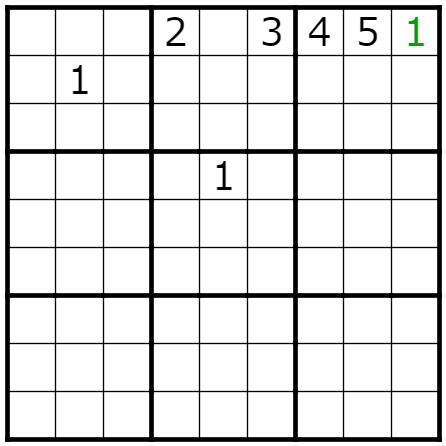
\includegraphics[keepaspectratio, scale=0.2]
      		{sample_rettumi_easy.png}
 	\caption{レッツミーの簡単な例}
 	\label{sample_rettumi_easy}
	\end{minipage}%
	\begin{minipage}[t]{0.5\columnwidth}
 	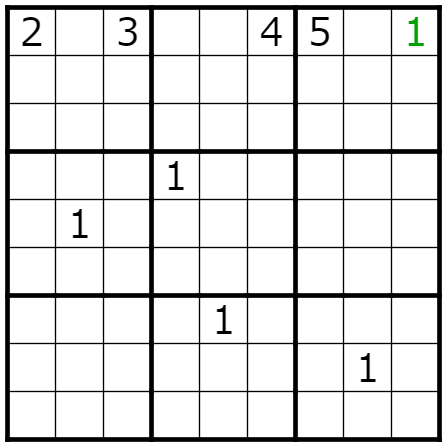
\includegraphics[keepaspectratio, scale=0.2]
      		{sample_rettumi_difficult.png}
 	\caption{レッツミーの難しい例}
 	\label{sample_rettumi_difficult}
	\end{minipage}
	\end{figure}

土手らの手法では問題24から84の問題がおおよそ70前後という難易度の値が大きくなった.これは,1つの数字に着目し,初級の手筋で入るブロックを探すといったことを1から9まで繰り返し行っていて,1つの数字に対する探索につき1加算する方法を取っており,それで埋まらなければ,残っている空白マスの数を難易度に加算して中級の手筋で解く,といった難易度付けをしているからである.具体的に動作を確認すると,中級手筋を使うまでに埋まった数字を調べるとおおよそが15個前後で,その時点での残りマスが50個前後であったため,今回の点数の付け方となっている.また,問題16,20の結果が41,45と他と違う値になった理由を調べたところ,加算した残りの空白マスの数が他の問題より少ない,つまり比較的盤面に数字が埋まったところで中級の手筋を使い出したためである.


\subsection{考察:上級問題}
表~\ref{study_hard}における問題32と36の提案手法の難易度に着目する.それぞれ7,10となっており,他の公式難易度 8 のものと比べると低くなっている.問題32の解法についてさらに考察を行うと,問題を解く過程で中級手筋の中でも難しい手筋であるマスミを使っていることが分かった.これにより,使用する上級手筋の種類や回数は少なくとも,途中で難しい中級手筋を使えば上級手筋の種類や回数が同等の問題よりも難易度が高くつけられている可能性がある.今回,中級手筋と上級手筋の難易度は格段に違うという理由から,上級問題での解法では中級以下の手筋には難易度 0 点と評価して計算している.しかし,上級手筋だけでなく中級手筋がどのように使われたかも加味すれば,より精度の高い難易度決定ができるかもしれない.

また,土手らの手法では同じ公式難易度でも点数が低い問題と高い問題のそれぞれが出力されている.これらの違いを調べてみると,例えば,難易度7の問題である問題4から20のうち,12番だけが他よりも高い値となっている.これは,12番以外の難易度7の問題は先に探索される2マスの表予約と裏予約のみ使って解ける問題であるのに対し,12番の問題はその後に探索されるいずれにしても理論を使わなければ解けない問題となっているからである.つまり,12番以外の問題は1種類の上級手筋の探索で終わるが,12番は2種類の上級手筋の探索をしなければならないので難易度が高くなっている.このように,同じ公式難易度でも使う手筋によって盤面を探索する回数に変化がある.土手らの手法では1つの手筋に対する1回の探索で少なくとも点数が54が上がるので,これにより難易度にばらつきが現れると考えられる.
また,土手らの手法では公式難易度7と8+で,難易度の差が変わらない問題がある.これは,難易度7の問題ではブロック内の2マスの表予約を使う問題があり,公式難易度8+の問題では列内の2マスの表予約を使う問題がある.本の難易度設定ではブロックよりも列にある予約の方が難しいとされているので後者の方が難しいとされているが,土手らの手法ではブロックの2マス表予約と列の2マス予約を同じ難易度と見なし1回の探索で同時に探索を行うため,難易度の差が変わっていないと考えられる.

また,上級手筋でも手筋の見えにくさというものがある.例えば,次のようなブロックでの3マスにおける表予約の成立時に顕著に出る.例えば\figref{sample_yoyaku_block3_easy}と\figref{sample_yoyaku_block3_difficult}はどちらもブロック内の3マスの表予約が成立している場合である.ここで,\figref{sample_yoyaku_block3_easy}では表予約を成立させている数字が上から1行目と左から1列目に固まっているので,この2つの列に注目すれば表予約が存在することに気づきやすい.しかし,\figref{sample_yoyaku_block3_difficult}では注目するべき列が上から1行目と2行目,左から1行目と2行目と先ほどの例よりも多い.さらに表予約が成立しているブロックに対して2行が効いている数字(ここでは1),2列が効いている数字(ここでは2),1行と1列が効いている数字(ここでは3)がある.どの数字もブロックに対しての数字の効き方が異なるので,この3つの数字が表予約を成立させていることに気づくのは前述の2列しか見なくてよい表予約よりも一般的に難しいとされている.
よって,先述したブロックでの3マスにおける表予約のように,手筋が成立しているマスの位置や,手筋成立に関わっている数字がある行や列を調べて,手筋に付ける難易度を変えるといった改善も考えられる.

	\begin{figure}[tb]
	\begin{minipage}[t]{0.5\columnwidth}
 	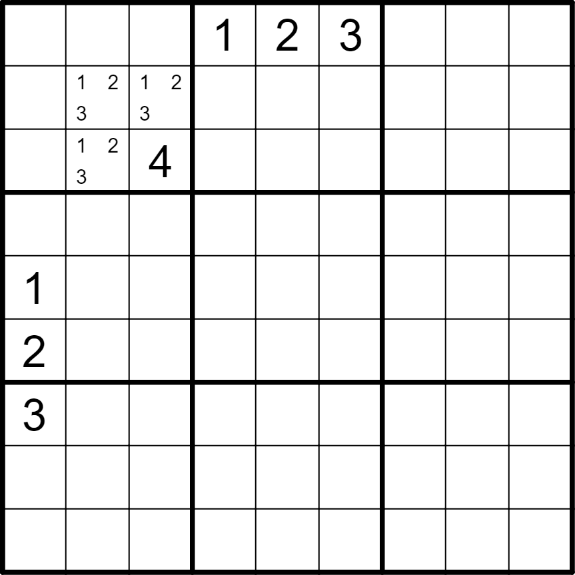
\includegraphics[keepaspectratio, scale=0.2]
      		{sample_yoyaku_block3_easy.png}
 	\caption{ブロック3マス表予約\\の簡単な例}
 	\label{sample_yoyaku_block3_easy}
	\end{minipage}%
	\begin{minipage}[t]{0.5\columnwidth}
 	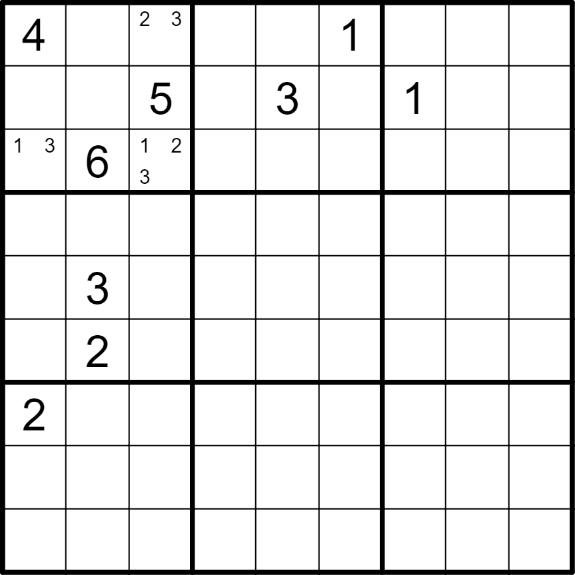
\includegraphics[keepaspectratio, scale=0.2]
      		{sample_yoyaku_block3_difficult.png}
 	\caption{ブロック3マス表予約\\の難しい例}
 	\label{sample_yoyaku_block3_difficult}
	\end{minipage}
	\end{figure}

\section{おわりに}
本稿では,数独に対する最も簡単な解法を見つけ,その解放を用いた問題の難易度を判定するソルバーを開発した.
今回,入力として与えた問題では,相関係数の結果や考察から既存手法よりも本研究による提案手法の方が公式難易度に近い難易度を目安として出せることが分かった.ただし,注意する点として,本研究では入力する問題が掲載されている本を出版社がどの手筋をどのような難易度で扱っているかをおおよその推測を行い,作成している.よって,他の出版社の本では今回とはまた違った結果になると考えられる.例えば,既存手法のように探索の回数の方を重点的に見るような指標で公式難易度が付けられている本であれば,既存手法の方が適切であろう.しかし,本研究の難易度設定とは違えど,それぞれの手筋に対して初級手筋,中級手筋など大まかな難易度付けが行われており,それに基づいて公式難易度が設定されているならば,本研究の手法が有効である可能性は高い.なぜなら,その難易度設定を元に各手筋の点数を決め,本研究の手法のように解法に点数を付けることで,それを難易度の目安とできるからである.

一方で,既存手法は決して本研究より悪い点ばかりではない.既存手法では,数字を探索する時の手間という,人間が解く時に難しいと感じる部分を点数で表している.今回作成した最も簡単な解法を見つける手法と,既存手法の探索の手間暇を数値化する手法,これらの良いバランスを取っている手法が今後出てくれば,数独の難易度決定はより安定し,より多くの人が納得できる難易度を付けやすくなるだろう.
今後の展望としては,初級問題に対する難易度決定ソルバーを実装していないため,実装して土井らの研究と比べてどのような結果になるのかを見てみたい.

また,今回の手法は他のペンシルパズルにも適用できる可能性がある.例えば,株式会社ニコリ社は数独以外の多くのペンシルパズルにおいても使われる手筋の難易度によって問題の難易度を決めている傾向にある.また,そうでなくてもインターネット上のサイトで出題されるようなパズルも,作者各々が持つ手筋の難易度によって問題の難易度を決めているのをよく見かける.よって,本研究のように最も簡単な解法を見つけて難易度を判定するようなソルバーが他のペンシルパズルに対しても実装できれば,そのパズルでも安定した難易度判定ができるであろう.


%\renewcommand{\bibname}{参考文献}

\bibliographystyle{junsrt}
\bibliography{bibsample}

\end{document}
